\chapter{Présentation générale sur l’agriculture sous Serres} \label{chap:Présentation générale sur l’agriculture sous Serres}

\section{Introduction}
L'agriculture sous serres est une méthode de production de cultures à l'aide de structures en plastique, en verre ou en polycarbonate pour créer un environnement contrôlé pour les plantes. Cette méthode est utilisée pour cultiver des plantes dans des environnements qui ne sont pas adaptés à leur croissance naturelle.
Les serres permettent également de contrôler les niveaux d'humidité, de température, de lumière et de ventilation, ce qui permet aux agriculteurs de produire des cultures tout au long de l'année, indépendamment des conditions météorologiques extérieures. Cette méthode de production de cultures est de plus en plus utilisée dans le monde entier pour répondre aux besoins alimentaires croissants de la population mondiale et pour assurer la sécurité alimentaire dans des conditions climatiques changeantes.
Bien que l'agriculture sous serres puisse offrir des avantages tels que des rendements plus élevés et une utilisation plus efficace des ressources.

\section{Tomates de serre }
La tomate est l'une des cultures les plus couramment cultivées sous serres en raison de sa rentabilité et de sa popularité auprès des consommateurs.Les serres permettent également de cultiver des variétés de tomates qui ne seraient pas viables dans des conditions extérieures. Les tomates de serre peuvent être cultivées tout au long de l'année, ce qui permet aux producteurs d'offrir des tomates fraîches en dehors de la saison de croissance traditionnelle.
La culture des tomates en serre est un moyen de production de tomates efficace et peu
coûteux en Algérie.
\begin{figure}
    \centering
    \label{fig:Exemple de calendrier de production de la tomate} 
    \caption{Exemple de calendrier de production de la tomate}
	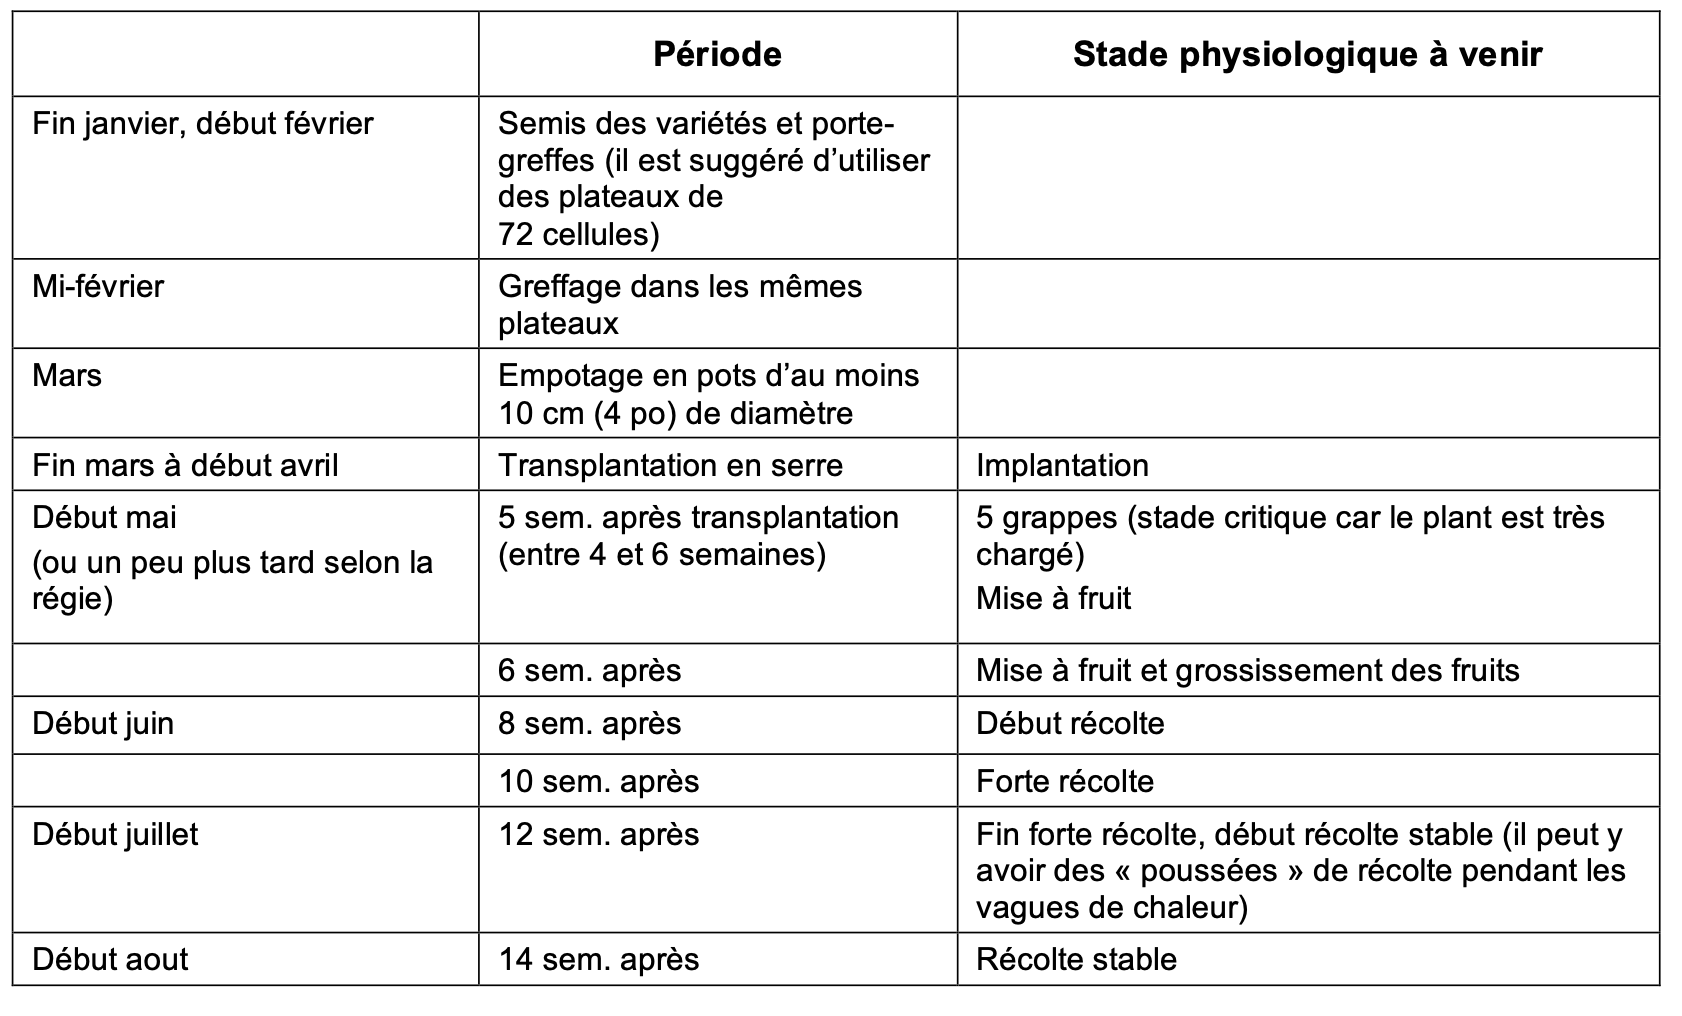
\includegraphics[width=15cm]{figures/periodetomate.png}
	
\end{figure}

\section{Caractéristiques}

\subsection{Température et Humidité}
Dans le rapport qui rédigé par Anne Weill et Jean Duval [3] exprime que 
La température est le facteur le plus déterminant dans la production de la tomate. Celle-ci
réagit énormément aux variations thermiques.
Un écart de température d’un ou deux degrés Celsius entre le jour et la nuit est favorable à
la production de fruits. Pour la production des plants et avant l’apparition des premières
fleurs, il est préférable toutefois de maintenir la température plus constante à environ
20 °C. En été, l’aération doit être suffisante pour que la température ne dépasse pas 28
°C. Idéalement, il ne faudrait pas que la température dépasse  25 °C, car au dessus de cette température la tomate ne fait plus aucun gain.L’humidité  devrait être
maintenue entre 60 et 80 \%. La culture elle-même génère beaucoup d’humidité et, par
conséquent, le taux d’humidité de la serre est souvent trop élevé. Il faut donc ventiler et
même souvent chauffer la serre pour déshumidifier.



\subsection{Lumière}
Eclairage
Comme il  explique dans l’article "Principes agronomiques de la tomate" [4]
Les tomates sont sensibles aux conditions de
faible luminosité. Elles exigent un minimum de 6 heures d’ensoleillement direct pour
fleurir. Toutefois, en cas de trop grande intensité du rayonnement solaire, des fentes, des
brûlures solaires et une coloration inégale peuvent apparaître au stade de maturité. Il est
donc essentiel, dans le cas des cultures sous serre, de s’assurer que les fruits disposent de
suffisamment d’ombre. La longueur du jour n’influence pas la production de tomates. Les
cultures sous serre sont par conséquent répandues sous un large éventail de latitudes.
\subsection{Sol}
En général, la tomate n'a pas d'exigences de sol. Cependant, elle s'adapte bien dans les sols profonds, meubles, bien aérés. Une texture sablonneuse ou sabloli-moneuse est préférable.
\subsection{Irrigation}
les tomates cultivées sous serre dépendront de l'arrosage que vous leur apporterez. Comme précisé Antoine de France Serres[5] L'arrosage est essentiel pour réussir vos cultures de tomates. Il doit être régulier, c'est-à-dire que vous ne devrez pas arroser beaucoup d'un coup puis plus du tout pendant une longue période au risque de voir les fruits éclater. Environ 2 ou 3 litres d'eau sont nécessaires chaque jour à vos plants.
Les apports en eau devront être plus importants entre la période de floraison et de développement des fruits. Un manque d'eau durant la phase de nouaison peut ruiner votre culture (la nouaison est la phase de formation initiale des fruits, lorsque l'ovaire de la fleur se transforme en fruit après fécondation). Au contraire, lorsque les tomates sont en phase de maturation, soit peu avant la récolte, vous devrez fortement limiter l'arrosage de façon à concentrer le goût et les saveurs de vos tomates.
Veillez à arroser vos plants au niveau des pieds, jamais au niveau du feuillage. Mouiller les feuilles pourrait conduire au développement de maladies.
Les systèmes de goutte à goutte sont un dispositif bien adapté pour la culture de tomates, car régulier et ciblé sur les pieds des plants. Laissez tout de même une certaine distance avec la base des plants de façon à optimiser le développement des racines en largeur.
\section{Conclusion}
En conclusion, les serres peuvent être utilisées pour produire des cultures de haute qualité, en particulier dans des environnements contrôlés où les conditions environnementales sont optimales pour la croissance des cultures. Les serres peuvent également être utilisées pour faire pousser des cultures plus rapidement et plus efficacement, augmentant ainsi la production alimentaire tout en réduisant les coûts. 
